\documentclass{article}
\usepackage{graphicx} % Required for inserting images
\usepackage{geometry}
\usepackage{setspace}
\geometry{total = {8.5in,11in}, margin= 1in}

\title{Gene Expression During the Covid-19 Pandemic}
\author{Seamus Stein}
\date{August 22, 2023}
\doublespacing

\begin{document}

\maketitle
\tableofcontents
\newpage
\section{Introduction}
The purpose of this study is to examine gene expression data for various genes and their relationship to other covariates during the COVID-19 pandemic \cite{Overmyer2021}. The gene expression data was linked to its metadata for analysis. In this study the covariates of interest are the age and sex of the patients as well as their ICU status. In this project the relationships will be examined by visualizing the data through the use of the ggplot2 package in R. In section 1.1 the biological function of \emph{APOM} gene which was selected for this study will be described. 

\subsection{\emph{APOM} Background}
The  gene that is of interest is the \emph{APOM} gene. The \emph{APOM} gene encodes a protein that is an apolipoprotein. The encoded protein is secreted through the plasma membrane but remains membrane-bound. It functions in the transportation of lipids. \cite{pubchem_apom_2023} 


In the following sections data will be presented on the \emph{LCN2} and \emph{APOA2} gene. The functions of these genes as well as the 10 genes that will be presented in the heatmap will not be discussed in this study.

\section{Subject Demographics and Clinical Characteristics}
Table \ref{Table1} presents the patient's demographics and clinical characteristics including summary statistics of the genes and covariate variables of interest in the study.

\begin{table}[h]
\centering
\begin{tabular}{lrl}

Variable                   & n = 74                    &  \\ \cline{1-2}
\textbf{ICU Status} n (\%)          &                            &  \\
\hspace{3mm} Not Admitted       & 25 (33.78)                 &  \\
\hspace{3mm} Admitted                   & 49 (66.22)                 &  \\
\textbf{Sex} n (\%)                 &                            &  \\
\hspace{3mm} Female                     & 25 (33.78)                 &  \\
\hspace{3mm} Male                       & 49 (66.22)                 &  \\

\textbf{Mechanical Ventilation} n (\%)                 &                            &  \\
\hspace{3mm} Not on Mechanical Ventilation & 36 (48.65) \\
\hspace{3mm} On Mechanical Ventilation & 38 (51.35) \\
\textbf{Age} Mean (sd)              & 63.31 (14.58)              &  \\
\textbf{Ferritin (ng/l)} Mean (sd)  & 834.26  (935.89)              &  \\
\textbf{Lactate (mmol/l)} Mean (sd)  & 0.95  (1.23)              &  \\
\textbf{APOM} Median {[}IQR{]}  & 3.29 {[}2.37, 4.53{]}      &  \\
\textbf{LCN2} Median {[}IQR{]}  & 136.43 {[}81.2, 586.76{]} &  \\
\textbf{APOA2} Median {[}IQR{]} & 0 {[}0, 0.2{]}             & \\ \cline{1-2}
\end{tabular}
\caption{\label{Table1} Subject Demographics and Clinical Characteristics}
\end{table}

\newpage
\section{Histogram of \emph{APOM} Expression}
\begin{figure}[h]
    \centering
    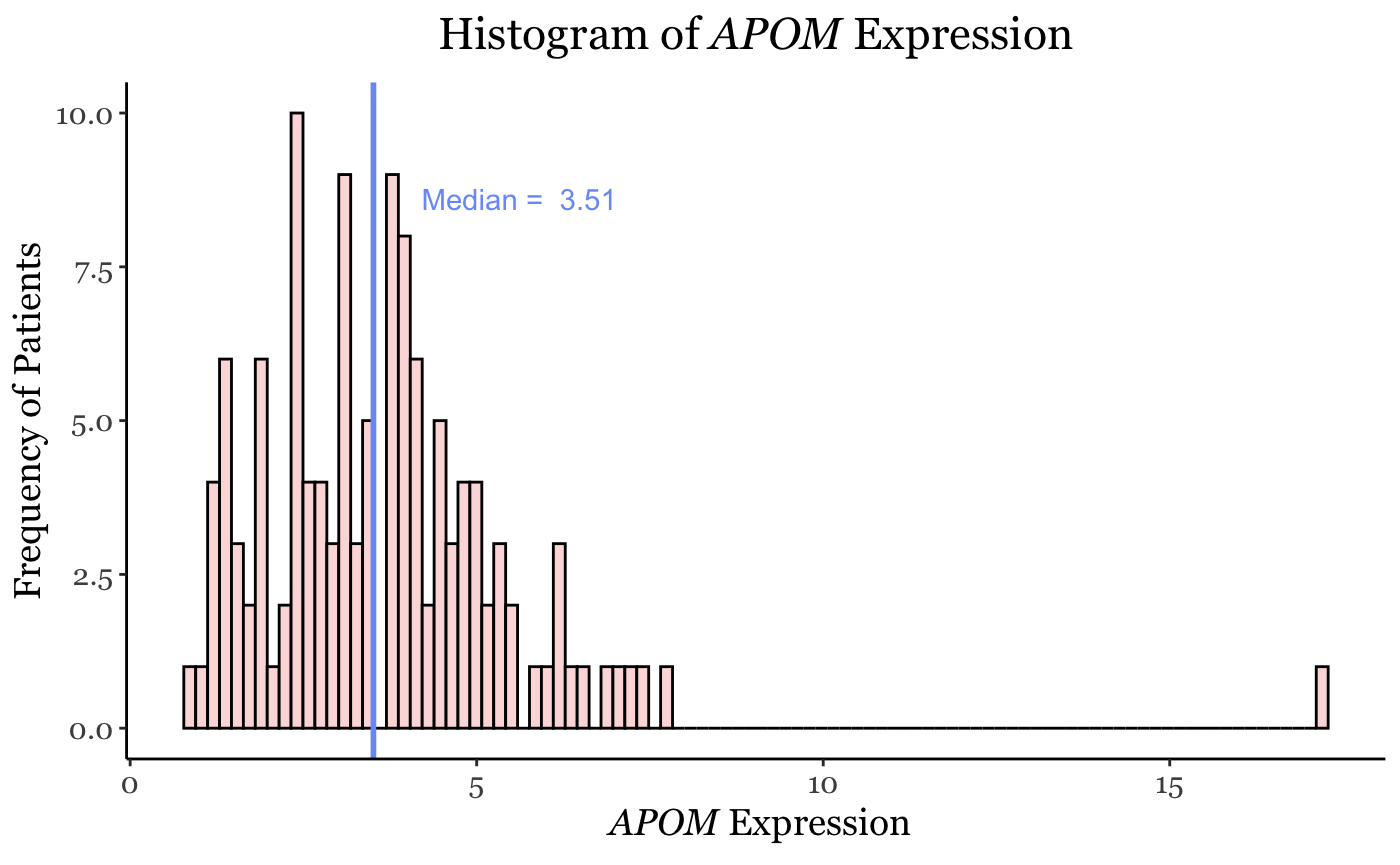
\includegraphics[width = \textwidth]{APOM_histogram.png}
    \caption{Histogram of \emph{APOM} Expression}
    \label{fig:APOMhist}
\end{figure}

\noindent When examining Figure \ref{fig:APOMhist} we notice that the the median \emph{APOM} expression level is 3.51. This is illustrated by the vertical line in the graph. As seen, the observed distribution of \emph{APOM} expression in the patients of the study is skewed to the right as there is a tail produced by the presence of the outlier on the right hand side of the graph.  
\newpage
\section{Scatter plot of \emph{APOM} Expression by Age}
Next, we will examine the relationship between age, the continuous variable of interest, and \emph{APOM} expression.
\begin{figure}[h]
    \centering
    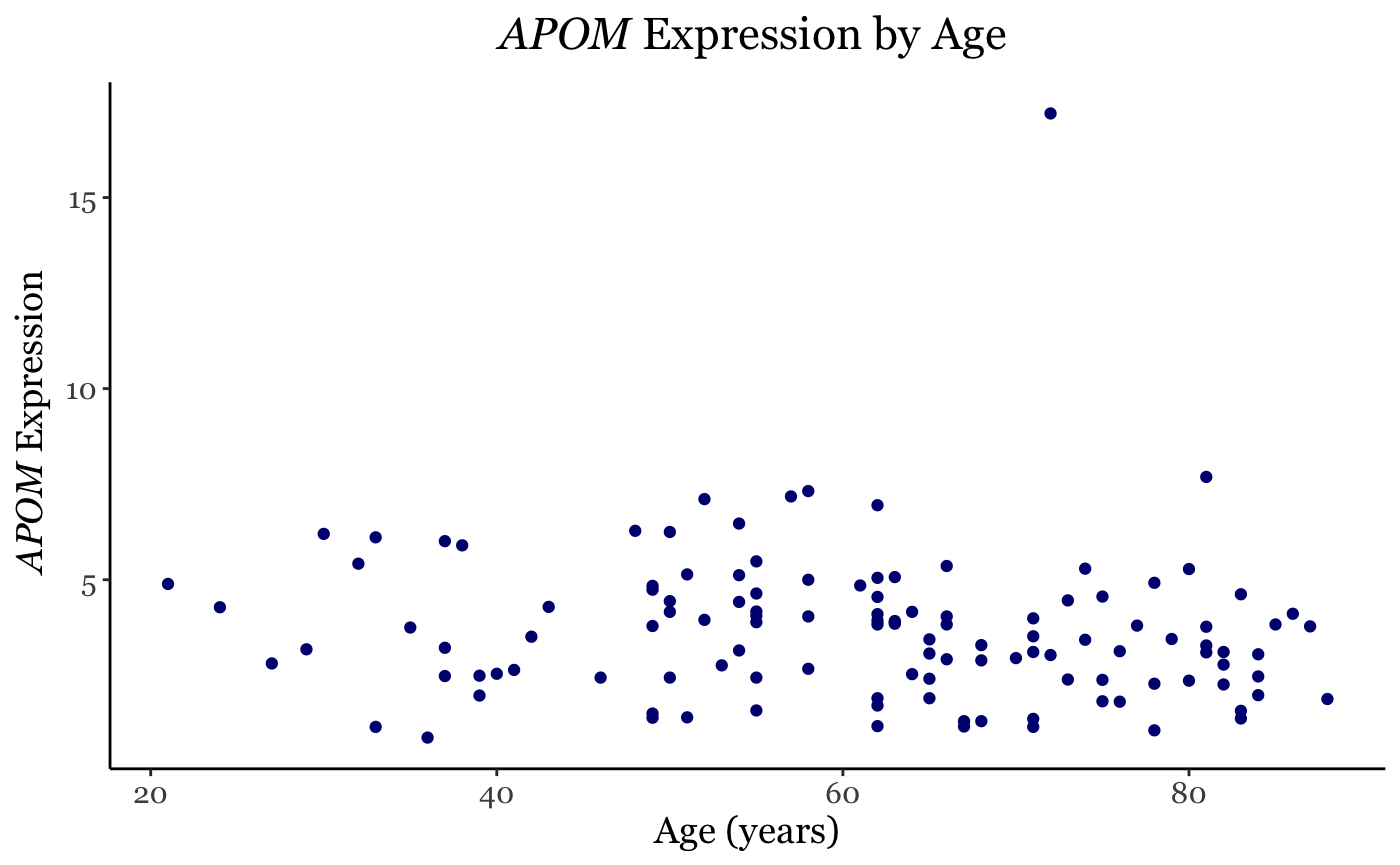
\includegraphics[width = \textwidth]{APOM_scatterplot.png}
    \caption{Scatter plot of \emph{APOM} Expression and Age}
    \label{fig:scatter}
\end{figure}

Figure \ref{fig:scatter} indicates that there is no relationship between age and \emph{APOM} expression. As age increases the expression of the \emph{APOM} gene does not increase or decrease. 

\section{Boxplot of \emph{APOM} Expression by ICU Status and Sex}
The third graph that will be examined is a boxplot. In this graph the \emph{APOM}'s gene expression will be examined by two categorical variables, sex and ICU status, respectively. In the analysis, there was a patient with an unknown in the sex variable. Since this could be interpreted as a missing value it was dropped from analysis. 
\newpage
\begin{figure}[h]
    \centering
    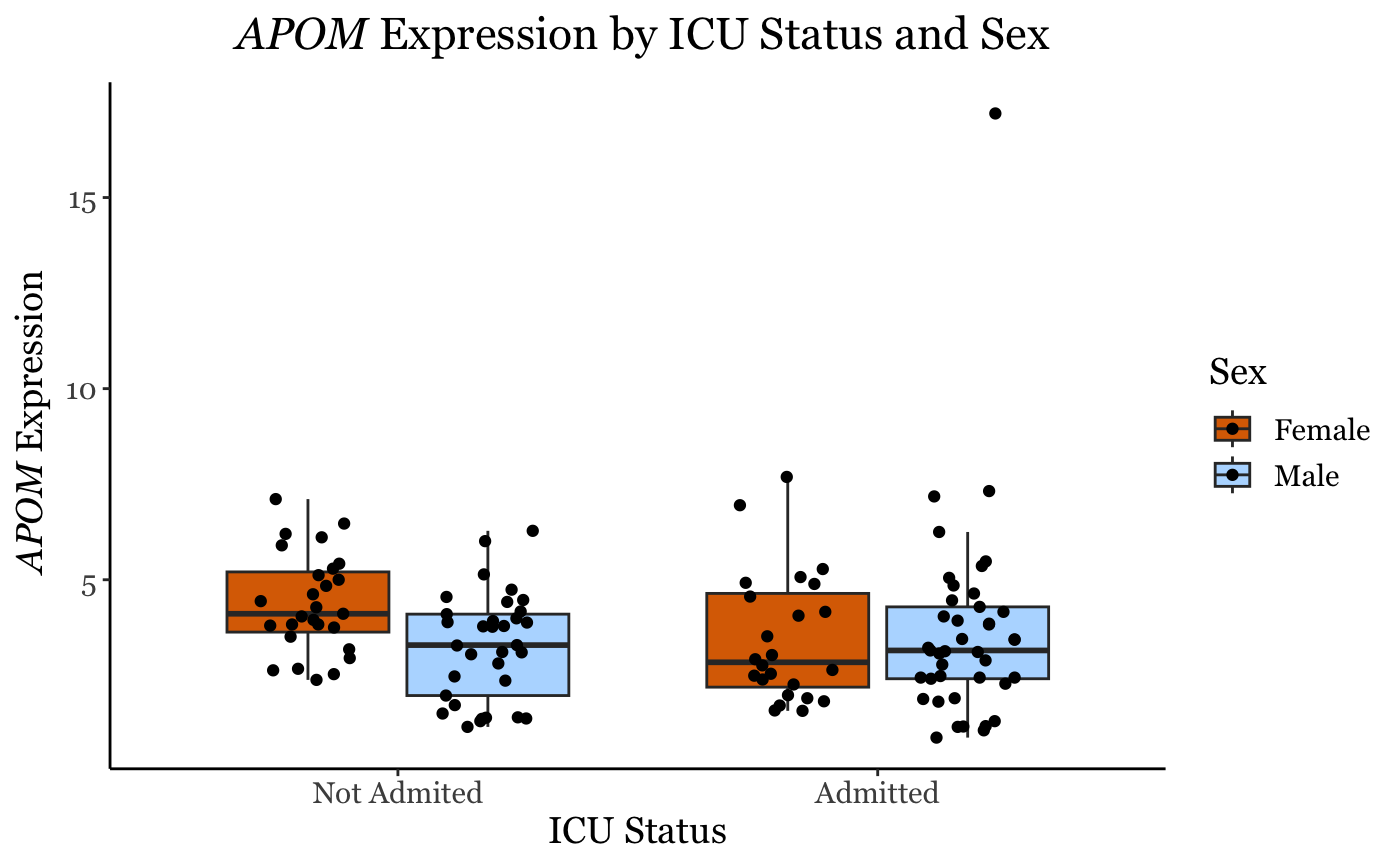
\includegraphics[width = \textwidth]{APOM_boxplot.png}
    \caption{Boxplot of\emph{APOM} Expression by ICU Status and Sex}
    \label{fig:boxplot}
\end{figure}


When examining Figure \ref{fig:boxplot}, it appears that among those who do are not admitted to the ICU the median of \emph{APOM} expression is greater among females compared to males. However, among those admitted to the ICU, the median level of expression is greater among males compared to females. The interquartile range for females is noticeably narrower for those not admitted to the ICU compared to those admitted to the ICU. Finally, there is an outlier, a male who was admitted to the ICU has an unusually high level of \emph{APOM} expression.

\section{Heatmap of Gene Expression}
In the following heatmap the expression 10 genes will be visualized. The genes that are considered include \emph{APOM}, \emph{LCN2}, \emph{APOA1}, \emph{APOA2}, \emph{MPO}, \emph{BPI}, \emph{DEFA1}, \emph{DEFA4}, \emph{PRTN3} and \emph{CTSG}. 
\newpage
\begin{figure}[h]
    \centering
    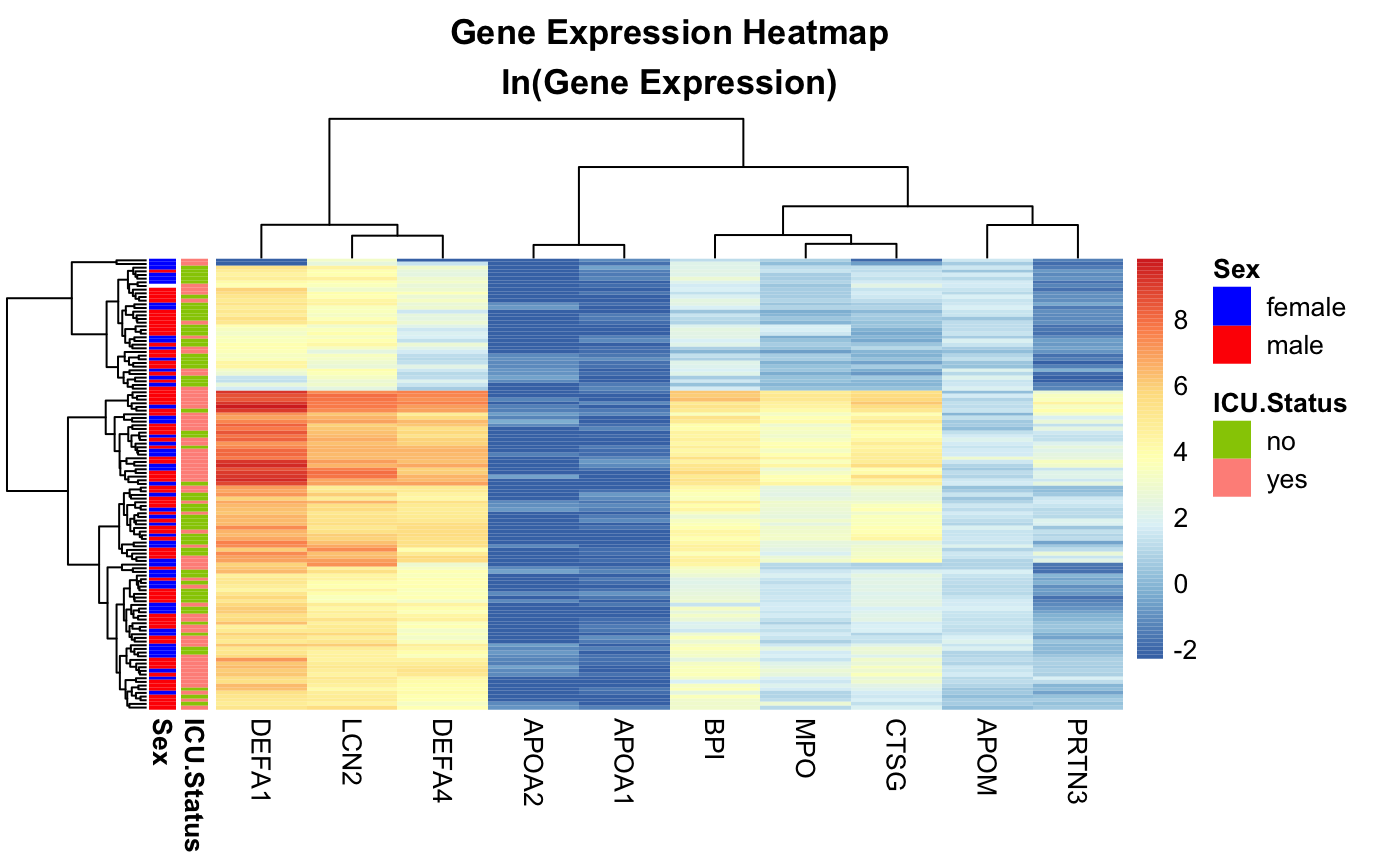
\includegraphics[width = \textwidth]{ln_heatmap.png}
    \caption{Heatmap of Log Transformed Gene Expression using the Euclidean Algorithm}
    \label{fig:heatmap}
\end{figure}

In Figure \ref{fig:heatmap} there are tracking bars for the two categorical variables of interest, sex and ICU status. The euclidean distance clustering algorithm was performed to create clusters of similar patient's with gene expression. The gene expression was log transformed by means of the natural log. When examining Figure \ref{fig:heatmap} many of the genes have low to medium gene expression in the clusters. The \emph{DEFA1} gene appears to have the greatest level of expression as it has the darkest color according to the tracking bar. When examining the summary statistics for the \emph{DEFA1} gene its maximum expression is 18863.9 or approximately 9.845 on the natural log scale. \emph{DEFA1}'s minimum expression is 0. This range is visualized by the heatmap tracking bar. The next greatest range of expression is found in the \emph{LCN2} gene (the minimum and maximum gene expression is 10.66 and 2928.23 respectively) followed by the \emph{DEFA4} gene (minimum expression is 0.0 and maximum expression is 1981.42). Compared to other genes selected, these genes had the greatest range of expression. 

\section{Raincloud Plot}
The final type of plot that will be examined is a raincloud plot. Figure \ref{fig:raincloud} displays a density of all the patients at particular levels of \emph{APOM} expression given by the x-axis. The expression levels are stratified by the patient's ICU status. Underneath each of the stratified density plots lies a horizontal bar plot. Created with a jitter, one can see for each strata where most of the patients lie. 

\begin{figure}[h]
    \centering
    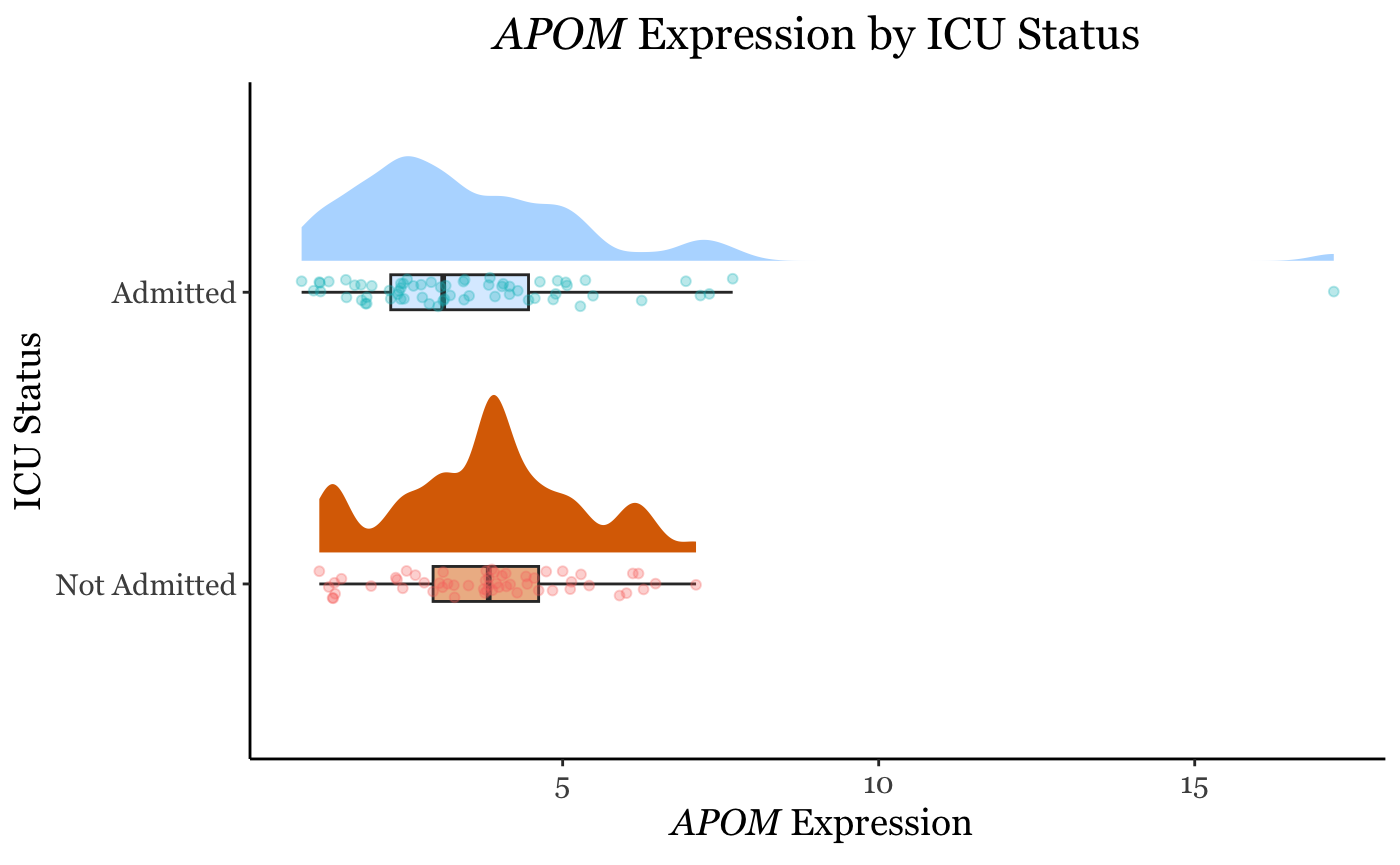
\includegraphics[width = \textwidth]{raincloud_apom.png}
    \caption{Raincloud Plot: \emph{APOM} Expression by ICU Status}
    \label{fig:raincloud}
\end{figure}

When examining Figure \ref{fig:raincloud}, for patients admitted to the ICU there is a greater density below the median resulting in a higher peak. This is in contrast to patients not admitted to the ICU where there is a greater amount of patients surrounding the median expression level for that strata. When comparing patients admitted to the ICU and those not admitted, those not admitted to the ICU appear to have a higher \emph{APOM} expression. It is important to note that this differs from \ref{fig:boxplot} in that we are not stratifying by the patient's sex.

Raincloud plots could be useful and further analysis could be done to compare the distribution of patients and density of expression in different genes of interest. One could also be interested in a different categorical variable and could expand the study to examine and compare and contrast expression levels, and resulting densities, of different genes by multiple categorical variables.

\section{Acknowledgements}
I would like to thank Graham who helped me create better bins on my histogram. I also would like to thank Elizabeth as we worked together on parts of our respective projects together. Other sources that I used when coding the project can be found in the references.\cite{baptiste_answer_2015}\cite{mcjudd_using_2015}\cite{noauthor_add_nodate}\cite{noauthor_graphics_nodate}\cite{noauthor_how_nodate}\cite{noauthor_solved-combining_nodate}

\bibliographystyle{pnas2009}
\bibliography{QBS103_refs}

\end{document}
